% Title: Block diagram of Third order noise shaper in Compact Disc Players
% Author: Ramón Jaramillo
\documentclass{article}

\usepackage{tikz}
%\usepackage{textcomp}
\begin{document}



\begin{figure}[t]
\centering
% Created by tikzDevice version 0.12 on 2019-05-07 15:15:52
% !TEX encoding = UTF-8 Unicode
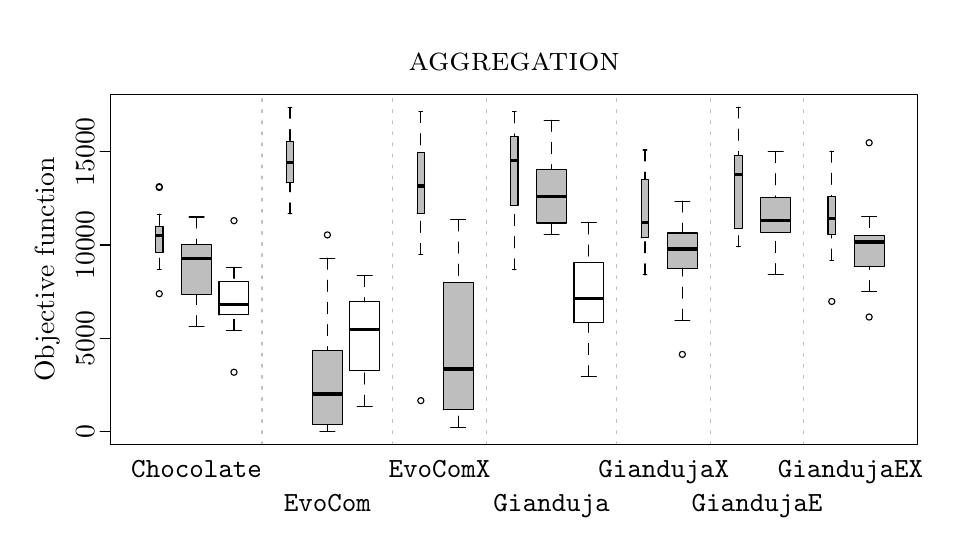
\begin{tikzpicture}[x=1pt,y=1pt]
\definecolor{fillColor}{RGB}{255,255,255}
\path[use as bounding box,fill=fillColor,fill opacity=0.00] (0,0) rectangle (325.21,180.67);
\begin{scope}
\path[clip] ( 30.00, 30.00) rectangle (321.61,156.67);
\definecolor{fillColor}{RGB}{190,190,190}

\path[fill=fillColor] ( 46.20, 99.54) --
	( 48.90, 99.54) --
	( 48.90,108.76) --
	( 46.20,108.76) --
	cycle;
\definecolor{drawColor}{RGB}{0,0,0}

\path[draw=drawColor,line width= 1.2pt,line join=round] ( 46.20,105.45) -- ( 48.90,105.45);

\path[draw=drawColor,line width= 0.4pt,dash pattern=on 4pt off 4pt ,line join=round,line cap=round] ( 47.55, 93.37) -- ( 47.55, 99.54);

\path[draw=drawColor,line width= 0.4pt,dash pattern=on 4pt off 4pt ,line join=round,line cap=round] ( 47.55,113.25) -- ( 47.55,108.76);

\path[draw=drawColor,line width= 0.4pt,line join=round,line cap=round] ( 46.88, 93.37) -- ( 48.23, 93.37);

\path[draw=drawColor,line width= 0.4pt,line join=round,line cap=round] ( 46.88,113.25) -- ( 48.23,113.25);

\path[draw=drawColor,line width= 0.4pt,line join=round,line cap=round] ( 46.20, 99.54) --
	( 48.90, 99.54) --
	( 48.90,108.76) --
	( 46.20,108.76) --
	( 46.20, 99.54);

\path[draw=drawColor,line width= 0.4pt,line join=round,line cap=round] ( 47.55, 84.53) circle (  1.12);

\path[draw=drawColor,line width= 0.4pt,line join=round,line cap=round] ( 47.55,123.22) circle (  1.12);

\path[draw=drawColor,line width= 0.4pt,line join=round,line cap=round] ( 47.55,122.94) circle (  1.12);

\path[fill=fillColor] ( 55.65, 84.30) --
	( 66.45, 84.30) --
	( 66.45,102.25) --
	( 55.65,102.25) --
	cycle;

\path[draw=drawColor,line width= 1.2pt,line join=round] ( 55.65, 97.16) -- ( 66.45, 97.16);

\path[draw=drawColor,line width= 0.4pt,dash pattern=on 4pt off 4pt ,line join=round,line cap=round] ( 61.05, 72.63) -- ( 61.05, 84.30);

\path[draw=drawColor,line width= 0.4pt,dash pattern=on 4pt off 4pt ,line join=round,line cap=round] ( 61.05,112.24) -- ( 61.05,102.25);

\path[draw=drawColor,line width= 0.4pt,line join=round,line cap=round] ( 58.35, 72.63) -- ( 63.75, 72.63);

\path[draw=drawColor,line width= 0.4pt,line join=round,line cap=round] ( 58.35,112.24) -- ( 63.75,112.24);

\path[draw=drawColor,line width= 0.4pt,line join=round,line cap=round] ( 55.65, 84.30) --
	( 66.45, 84.30) --
	( 66.45,102.25) --
	( 55.65,102.25) --
	( 55.65, 84.30);
\definecolor{fillColor}{RGB}{255,255,255}

\path[fill=fillColor] ( 69.15, 76.88) --
	( 79.95, 76.88) --
	( 79.95, 88.86) --
	( 69.15, 88.86) --
	cycle;

\path[draw=drawColor,line width= 1.2pt,line join=round] ( 69.15, 80.73) -- ( 79.95, 80.73);

\path[draw=drawColor,line width= 0.4pt,dash pattern=on 4pt off 4pt ,line join=round,line cap=round] ( 74.55, 71.28) -- ( 74.55, 76.88);

\path[draw=drawColor,line width= 0.4pt,dash pattern=on 4pt off 4pt ,line join=round,line cap=round] ( 74.55, 94.09) -- ( 74.55, 88.86);

\path[draw=drawColor,line width= 0.4pt,line join=round,line cap=round] ( 71.85, 71.28) -- ( 77.25, 71.28);

\path[draw=drawColor,line width= 0.4pt,line join=round,line cap=round] ( 71.85, 94.09) -- ( 77.25, 94.09);

\path[draw=drawColor,line width= 0.4pt,line join=round,line cap=round] ( 69.15, 76.88) --
	( 79.95, 76.88) --
	( 79.95, 88.86) --
	( 69.15, 88.86) --
	( 69.15, 76.88);

\path[draw=drawColor,line width= 0.4pt,line join=round,line cap=round] ( 74.55, 56.16) circle (  1.12);

\path[draw=drawColor,line width= 0.4pt,line join=round,line cap=round] ( 74.55,110.93) circle (  1.12);
\definecolor{fillColor}{RGB}{190,190,190}

\path[fill=fillColor] ( 93.45,124.61) --
	( 96.15,124.61) --
	( 96.15,139.52) --
	( 93.45,139.52) --
	cycle;

\path[draw=drawColor,line width= 1.2pt,line join=round] ( 93.45,132.00) -- ( 96.15,132.00);

\path[draw=drawColor,line width= 0.4pt,dash pattern=on 4pt off 4pt ,line join=round,line cap=round] ( 94.80,113.38) -- ( 94.80,124.61);

\path[draw=drawColor,line width= 0.4pt,dash pattern=on 4pt off 4pt ,line join=round,line cap=round] ( 94.80,151.91) -- ( 94.80,139.52);

\path[draw=drawColor,line width= 0.4pt,line join=round,line cap=round] ( 94.13,113.38) -- ( 95.48,113.38);

\path[draw=drawColor,line width= 0.4pt,line join=round,line cap=round] ( 94.13,151.91) -- ( 95.48,151.91);

\path[draw=drawColor,line width= 0.4pt,line join=round,line cap=round] ( 93.45,124.61) --
	( 96.15,124.61) --
	( 96.15,139.52) --
	( 93.45,139.52) --
	( 93.45,124.61);

\path[fill=fillColor] (102.90, 37.23) --
	(113.70, 37.23) --
	(113.70, 64.06) --
	(102.90, 64.06) --
	cycle;

\path[draw=drawColor,line width= 1.2pt,line join=round] (102.90, 48.35) -- (113.70, 48.35);

\path[draw=drawColor,line width= 0.4pt,dash pattern=on 4pt off 4pt ,line join=round,line cap=round] (108.30, 34.69) -- (108.30, 37.23);

\path[draw=drawColor,line width= 0.4pt,dash pattern=on 4pt off 4pt ,line join=round,line cap=round] (108.30, 97.39) -- (108.30, 64.06);

\path[draw=drawColor,line width= 0.4pt,line join=round,line cap=round] (105.60, 34.69) -- (111.00, 34.69);

\path[draw=drawColor,line width= 0.4pt,line join=round,line cap=round] (105.60, 97.39) -- (111.00, 97.39);

\path[draw=drawColor,line width= 0.4pt,line join=round,line cap=round] (102.90, 37.23) --
	(113.70, 37.23) --
	(113.70, 64.06) --
	(102.90, 64.06) --
	(102.90, 37.23);

\path[draw=drawColor,line width= 0.4pt,line join=round,line cap=round] (108.30,105.79) circle (  1.12);
\definecolor{fillColor}{RGB}{255,255,255}

\path[fill=fillColor] (116.40, 56.73) --
	(127.20, 56.73) --
	(127.20, 81.60) --
	(116.40, 81.60) --
	cycle;

\path[draw=drawColor,line width= 1.2pt,line join=round] (116.40, 71.65) -- (127.20, 71.65);

\path[draw=drawColor,line width= 0.4pt,dash pattern=on 4pt off 4pt ,line join=round,line cap=round] (121.80, 43.91) -- (121.80, 56.73);

\path[draw=drawColor,line width= 0.4pt,dash pattern=on 4pt off 4pt ,line join=round,line cap=round] (121.80, 91.11) -- (121.80, 81.60);

\path[draw=drawColor,line width= 0.4pt,line join=round,line cap=round] (119.10, 43.91) -- (124.50, 43.91);

\path[draw=drawColor,line width= 0.4pt,line join=round,line cap=round] (119.10, 91.11) -- (124.50, 91.11);

\path[draw=drawColor,line width= 0.4pt,line join=round,line cap=round] (116.40, 56.73) --
	(127.20, 56.73) --
	(127.20, 81.60) --
	(116.40, 81.60) --
	(116.40, 56.73);
\definecolor{fillColor}{RGB}{190,190,190}

\path[fill=fillColor] (140.71,113.56) --
	(143.41,113.56) --
	(143.41,135.60) --
	(140.71,135.60) --
	cycle;

\path[draw=drawColor,line width= 1.2pt,line join=round] (140.71,123.42) -- (143.41,123.42);

\path[draw=drawColor,line width= 0.4pt,dash pattern=on 4pt off 4pt ,line join=round,line cap=round] (142.06, 98.71) -- (142.06,113.56);

\path[draw=drawColor,line width= 0.4pt,dash pattern=on 4pt off 4pt ,line join=round,line cap=round] (142.06,150.34) -- (142.06,135.60);

\path[draw=drawColor,line width= 0.4pt,line join=round,line cap=round] (141.38, 98.71) -- (142.73, 98.71);

\path[draw=drawColor,line width= 0.4pt,line join=round,line cap=round] (141.38,150.34) -- (142.73,150.34);

\path[draw=drawColor,line width= 0.4pt,line join=round,line cap=round] (140.71,113.56) --
	(143.41,113.56) --
	(143.41,135.60) --
	(140.71,135.60) --
	(140.71,113.56);

\path[draw=drawColor,line width= 0.4pt,line join=round,line cap=round] (142.06, 45.90) circle (  1.12);

\path[fill=fillColor] (150.16, 42.58) --
	(160.96, 42.58) --
	(160.96, 88.47) --
	(150.16, 88.47) --
	cycle;

\path[draw=drawColor,line width= 1.2pt,line join=round] (150.16, 57.36) -- (160.96, 57.36);

\path[draw=drawColor,line width= 0.4pt,dash pattern=on 4pt off 4pt ,line join=round,line cap=round] (155.56, 36.32) -- (155.56, 42.58);

\path[draw=drawColor,line width= 0.4pt,dash pattern=on 4pt off 4pt ,line join=round,line cap=round] (155.56,111.21) -- (155.56, 88.47);

\path[draw=drawColor,line width= 0.4pt,line join=round,line cap=round] (152.86, 36.32) -- (158.26, 36.32);

\path[draw=drawColor,line width= 0.4pt,line join=round,line cap=round] (152.86,111.21) -- (158.26,111.21);

\path[draw=drawColor,line width= 0.4pt,line join=round,line cap=round] (150.16, 42.58) --
	(160.96, 42.58) --
	(160.96, 88.47) --
	(150.16, 88.47) --
	(150.16, 42.58);

\path[fill=fillColor] (174.46,116.57) --
	(177.16,116.57) --
	(177.16,141.42) --
	(174.46,141.42) --
	cycle;

\path[draw=drawColor,line width= 1.2pt,line join=round] (174.46,132.60) -- (177.16,132.60);

\path[draw=drawColor,line width= 0.4pt,dash pattern=on 4pt off 4pt ,line join=round,line cap=round] (175.81, 93.15) -- (175.81,116.57);

\path[draw=drawColor,line width= 0.4pt,dash pattern=on 4pt off 4pt ,line join=round,line cap=round] (175.81,150.31) -- (175.81,141.42);

\path[draw=drawColor,line width= 0.4pt,line join=round,line cap=round] (175.13, 93.15) -- (176.48, 93.15);

\path[draw=drawColor,line width= 0.4pt,line join=round,line cap=round] (175.13,150.31) -- (176.48,150.31);

\path[draw=drawColor,line width= 0.4pt,line join=round,line cap=round] (174.46,116.57) --
	(177.16,116.57) --
	(177.16,141.42) --
	(174.46,141.42) --
	(174.46,116.57);

\path[fill=fillColor] (183.91,110.08) --
	(194.71,110.08) --
	(194.71,129.38) --
	(183.91,129.38) --
	cycle;

\path[draw=drawColor,line width= 1.2pt,line join=round] (183.91,119.54) -- (194.71,119.54);

\path[draw=drawColor,line width= 0.4pt,dash pattern=on 4pt off 4pt ,line join=round,line cap=round] (189.31,106.06) -- (189.31,110.08);

\path[draw=drawColor,line width= 0.4pt,dash pattern=on 4pt off 4pt ,line join=round,line cap=round] (189.31,147.20) -- (189.31,129.38);

\path[draw=drawColor,line width= 0.4pt,line join=round,line cap=round] (186.61,106.06) -- (192.01,106.06);

\path[draw=drawColor,line width= 0.4pt,line join=round,line cap=round] (186.61,147.20) -- (192.01,147.20);

\path[draw=drawColor,line width= 0.4pt,line join=round,line cap=round] (183.91,110.08) --
	(194.71,110.08) --
	(194.71,129.38) --
	(183.91,129.38) --
	(183.91,110.08);
\definecolor{fillColor}{RGB}{255,255,255}

\path[fill=fillColor] (197.41, 74.03) --
	(208.21, 74.03) --
	(208.21, 95.88) --
	(197.41, 95.88) --
	cycle;

\path[draw=drawColor,line width= 1.2pt,line join=round] (197.41, 82.80) -- (208.21, 82.80);

\path[draw=drawColor,line width= 0.4pt,dash pattern=on 4pt off 4pt ,line join=round,line cap=round] (202.81, 54.56) -- (202.81, 74.03);

\path[draw=drawColor,line width= 0.4pt,dash pattern=on 4pt off 4pt ,line join=round,line cap=round] (202.81,110.12) -- (202.81, 95.88);

\path[draw=drawColor,line width= 0.4pt,line join=round,line cap=round] (200.11, 54.56) -- (205.51, 54.56);

\path[draw=drawColor,line width= 0.4pt,line join=round,line cap=round] (200.11,110.12) -- (205.51,110.12);

\path[draw=drawColor,line width= 0.4pt,line join=round,line cap=round] (197.41, 74.03) --
	(208.21, 74.03) --
	(208.21, 95.88) --
	(197.41, 95.88) --
	(197.41, 74.03);
\definecolor{fillColor}{RGB}{190,190,190}

\path[fill=fillColor] (221.71,104.69) --
	(224.41,104.69) --
	(224.41,125.79) --
	(221.71,125.79) --
	cycle;

\path[draw=drawColor,line width= 1.2pt,line join=round] (221.71,110.26) -- (224.41,110.26);

\path[draw=drawColor,line width= 0.4pt,dash pattern=on 4pt off 4pt ,line join=round,line cap=round] (223.06, 91.33) -- (223.06,104.69);

\path[draw=drawColor,line width= 0.4pt,dash pattern=on 4pt off 4pt ,line join=round,line cap=round] (223.06,136.47) -- (223.06,125.79);

\path[draw=drawColor,line width= 0.4pt,line join=round,line cap=round] (222.38, 91.33) -- (223.73, 91.33);

\path[draw=drawColor,line width= 0.4pt,line join=round,line cap=round] (222.38,136.47) -- (223.73,136.47);

\path[draw=drawColor,line width= 0.4pt,line join=round,line cap=round] (221.71,104.69) --
	(224.41,104.69) --
	(224.41,125.79) --
	(221.71,125.79) --
	(221.71,104.69);

\path[fill=fillColor] (231.16, 93.75) --
	(241.96, 93.75) --
	(241.96,106.47) --
	(231.16,106.47) --
	cycle;

\path[draw=drawColor,line width= 1.2pt,line join=round] (231.16,100.65) -- (241.96,100.65);

\path[draw=drawColor,line width= 0.4pt,dash pattern=on 4pt off 4pt ,line join=round,line cap=round] (236.56, 74.91) -- (236.56, 93.75);

\path[draw=drawColor,line width= 0.4pt,dash pattern=on 4pt off 4pt ,line join=round,line cap=round] (236.56,118.01) -- (236.56,106.47);

\path[draw=drawColor,line width= 0.4pt,line join=round,line cap=round] (233.86, 74.91) -- (239.26, 74.91);

\path[draw=drawColor,line width= 0.4pt,line join=round,line cap=round] (233.86,118.01) -- (239.26,118.01);

\path[draw=drawColor,line width= 0.4pt,line join=round,line cap=round] (231.16, 93.75) --
	(241.96, 93.75) --
	(241.96,106.47) --
	(231.16,106.47) --
	(231.16, 93.75);

\path[draw=drawColor,line width= 0.4pt,line join=round,line cap=round] (236.56, 62.61) circle (  1.12);

\path[fill=fillColor] (255.46,108.03) --
	(258.16,108.03) --
	(258.16,134.53) --
	(255.46,134.53) --
	cycle;

\path[draw=drawColor,line width= 1.2pt,line join=round] (255.46,127.50) -- (258.16,127.50);

\path[draw=drawColor,line width= 0.4pt,dash pattern=on 4pt off 4pt ,line join=round,line cap=round] (256.81,101.51) -- (256.81,108.03);

\path[draw=drawColor,line width= 0.4pt,dash pattern=on 4pt off 4pt ,line join=round,line cap=round] (256.81,151.98) -- (256.81,134.53);

\path[draw=drawColor,line width= 0.4pt,line join=round,line cap=round] (256.14,101.51) -- (257.49,101.51);

\path[draw=drawColor,line width= 0.4pt,line join=round,line cap=round] (256.14,151.98) -- (257.49,151.98);

\path[draw=drawColor,line width= 0.4pt,line join=round,line cap=round] (255.46,108.03) --
	(258.16,108.03) --
	(258.16,134.53) --
	(255.46,134.53) --
	(255.46,108.03);

\path[fill=fillColor] (264.91,106.81) --
	(275.71,106.81) --
	(275.71,119.24) --
	(264.91,119.24) --
	cycle;

\path[draw=drawColor,line width= 1.2pt,line join=round] (264.91,110.88) -- (275.71,110.88);

\path[draw=drawColor,line width= 0.4pt,dash pattern=on 4pt off 4pt ,line join=round,line cap=round] (270.31, 91.41) -- (270.31,106.81);

\path[draw=drawColor,line width= 0.4pt,dash pattern=on 4pt off 4pt ,line join=round,line cap=round] (270.31,135.89) -- (270.31,119.24);

\path[draw=drawColor,line width= 0.4pt,line join=round,line cap=round] (267.61, 91.41) -- (273.01, 91.41);

\path[draw=drawColor,line width= 0.4pt,line join=round,line cap=round] (267.61,135.89) -- (273.01,135.89);

\path[draw=drawColor,line width= 0.4pt,line join=round,line cap=round] (264.91,106.81) --
	(275.71,106.81) --
	(275.71,119.24) --
	(264.91,119.24) --
	(264.91,106.81);

\path[fill=fillColor] (289.21,105.90) --
	(291.91,105.90) --
	(291.91,119.68) --
	(289.21,119.68) --
	cycle;

\path[draw=drawColor,line width= 1.2pt,line join=round] (289.21,111.67) -- (291.91,111.67);

\path[draw=drawColor,line width= 0.4pt,dash pattern=on 4pt off 4pt ,line join=round,line cap=round] (290.56, 96.68) -- (290.56,105.90);

\path[draw=drawColor,line width= 0.4pt,dash pattern=on 4pt off 4pt ,line join=round,line cap=round] (290.56,136.05) -- (290.56,119.68);

\path[draw=drawColor,line width= 0.4pt,line join=round,line cap=round] (289.89, 96.68) -- (291.24, 96.68);

\path[draw=drawColor,line width= 0.4pt,line join=round,line cap=round] (289.89,136.05) -- (291.24,136.05);

\path[draw=drawColor,line width= 0.4pt,line join=round,line cap=round] (289.21,105.90) --
	(291.91,105.90) --
	(291.91,119.68) --
	(289.21,119.68) --
	(289.21,105.90);

\path[draw=drawColor,line width= 0.4pt,line join=round,line cap=round] (290.56, 81.74) circle (  1.12);

\path[fill=fillColor] (298.66, 94.52) --
	(309.46, 94.52) --
	(309.46,105.71) --
	(298.66,105.71) --
	cycle;

\path[draw=drawColor,line width= 1.2pt,line join=round] (298.66,103.24) -- (309.46,103.24);

\path[draw=drawColor,line width= 0.4pt,dash pattern=on 4pt off 4pt ,line join=round,line cap=round] (304.06, 85.30) -- (304.06, 94.52);

\path[draw=drawColor,line width= 0.4pt,dash pattern=on 4pt off 4pt ,line join=round,line cap=round] (304.06,112.42) -- (304.06,105.71);

\path[draw=drawColor,line width= 0.4pt,line join=round,line cap=round] (301.36, 85.30) -- (306.76, 85.30);

\path[draw=drawColor,line width= 0.4pt,line join=round,line cap=round] (301.36,112.42) -- (306.76,112.42);

\path[draw=drawColor,line width= 0.4pt,line join=round,line cap=round] (298.66, 94.52) --
	(309.46, 94.52) --
	(309.46,105.71) --
	(298.66,105.71) --
	(298.66, 94.52);

\path[draw=drawColor,line width= 0.4pt,line join=round,line cap=round] (304.06, 76.11) circle (  1.12);

\path[draw=drawColor,line width= 0.4pt,line join=round,line cap=round] (304.06,139.09) circle (  1.12);
\definecolor{drawColor}{RGB}{190,190,190}

\path[draw=drawColor,line width= 0.4pt,dash pattern=on 1pt off 3pt ,line join=round,line cap=round] ( 84.68, 30.00) -- ( 84.68,156.67);

\path[draw=drawColor,line width= 0.4pt,dash pattern=on 1pt off 3pt ,line join=round,line cap=round] (131.93, 30.00) -- (131.93,156.67);

\path[draw=drawColor,line width= 0.4pt,dash pattern=on 1pt off 3pt ,line join=round,line cap=round] (165.68, 30.00) -- (165.68,156.67);

\path[draw=drawColor,line width= 0.4pt,dash pattern=on 1pt off 3pt ,line join=round,line cap=round] (212.93, 30.00) -- (212.93,156.67);

\path[draw=drawColor,line width= 0.4pt,dash pattern=on 1pt off 3pt ,line join=round,line cap=round] (246.69, 30.00) -- (246.69,156.67);

\path[draw=drawColor,line width= 0.4pt,dash pattern=on 1pt off 3pt ,line join=round,line cap=round] (280.44, 30.00) -- (280.44,156.67);
\end{scope}
\begin{scope}
\path[clip] (  0.00,  0.00) rectangle (325.21,180.67);
\definecolor{drawColor}{RGB}{0,0,0}

\node[text=drawColor,anchor=base,inner sep=0pt, outer sep=0pt, scale=  1.00] at ( 61.05, 18.00) {\texttt{Chocolate}};

\node[text=drawColor,anchor=base,inner sep=0pt, outer sep=0pt, scale=  1.00] at (148.81, 18.00) {\texttt{EvoComX}};

\node[text=drawColor,anchor=base,inner sep=0pt, outer sep=0pt, scale=  1.00] at (229.81, 18.00) {\texttt{GiandujaX}};

\node[text=drawColor,anchor=base,inner sep=0pt, outer sep=0pt, scale=  1.00] at (297.31, 18.00) {\texttt{GiandujaEX}};

\node[text=drawColor,anchor=base,inner sep=0pt, outer sep=0pt, scale=  1.00] at (108.30,  6.00) {\texttt{EvoCom}};

\node[text=drawColor,anchor=base,inner sep=0pt, outer sep=0pt, scale=  1.00] at (189.31,  6.00) {\texttt{Gianduja}};

\node[text=drawColor,anchor=base,inner sep=0pt, outer sep=0pt, scale=  1.00] at (263.56,  6.00) {\texttt{GiandujaE}};
\end{scope}
\begin{scope}
\path[clip] (  0.00,  0.00) rectangle (325.21,180.67);
\definecolor{drawColor}{RGB}{0,0,0}

\node[text=drawColor,anchor=base,inner sep=0pt, outer sep=0pt, scale=  1.20] at (175.81,165.07) {\textsc{aggregation}};

\node[text=drawColor,rotate= 90.00,anchor=base,inner sep=0pt, outer sep=0pt, scale=  1.00] at (  9.60, 93.34) {Objective function};
\end{scope}
\begin{scope}
\path[clip] (  0.00,  0.00) rectangle (325.21,180.67);
\definecolor{drawColor}{RGB}{0,0,0}

\path[draw=drawColor,line width= 0.4pt,line join=round,line cap=round] ( 30.00, 34.69) -- ( 30.00,135.83);

\path[draw=drawColor,line width= 0.4pt,line join=round,line cap=round] ( 30.00, 34.69) -- ( 26.20, 34.69);

\path[draw=drawColor,line width= 0.4pt,line join=round,line cap=round] ( 30.00, 68.41) -- ( 26.20, 68.41);

\path[draw=drawColor,line width= 0.4pt,line join=round,line cap=round] ( 30.00,102.12) -- ( 26.20,102.12);

\path[draw=drawColor,line width= 0.4pt,line join=round,line cap=round] ( 30.00,135.83) -- ( 26.20,135.83);

\node[text=drawColor,rotate= 90.00,anchor=base,inner sep=0pt, outer sep=0pt, scale=  1.00] at ( 24.00, 34.69) {0};

\node[text=drawColor,rotate= 90.00,anchor=base,inner sep=0pt, outer sep=0pt, scale=  1.00] at ( 24.00, 68.41) {5000};

\node[text=drawColor,rotate= 90.00,anchor=base,inner sep=0pt, outer sep=0pt, scale=  1.00] at ( 24.00,102.12) {10000};

\node[text=drawColor,rotate= 90.00,anchor=base,inner sep=0pt, outer sep=0pt, scale=  1.00] at ( 24.00,135.83) {15000};

\path[draw=drawColor,line width= 0.4pt,line join=round,line cap=round] ( 30.00, 30.00) --
	(321.61, 30.00) --
	(321.61,156.67) --
	( 30.00,156.67) --
	( 30.00, 30.00);
\end{scope}
\end{tikzpicture}

\hfill
% Created by tikzDevice version 0.11 on 2018-04-09 15:27:55
% !TEX encoding = UTF-8 Unicode
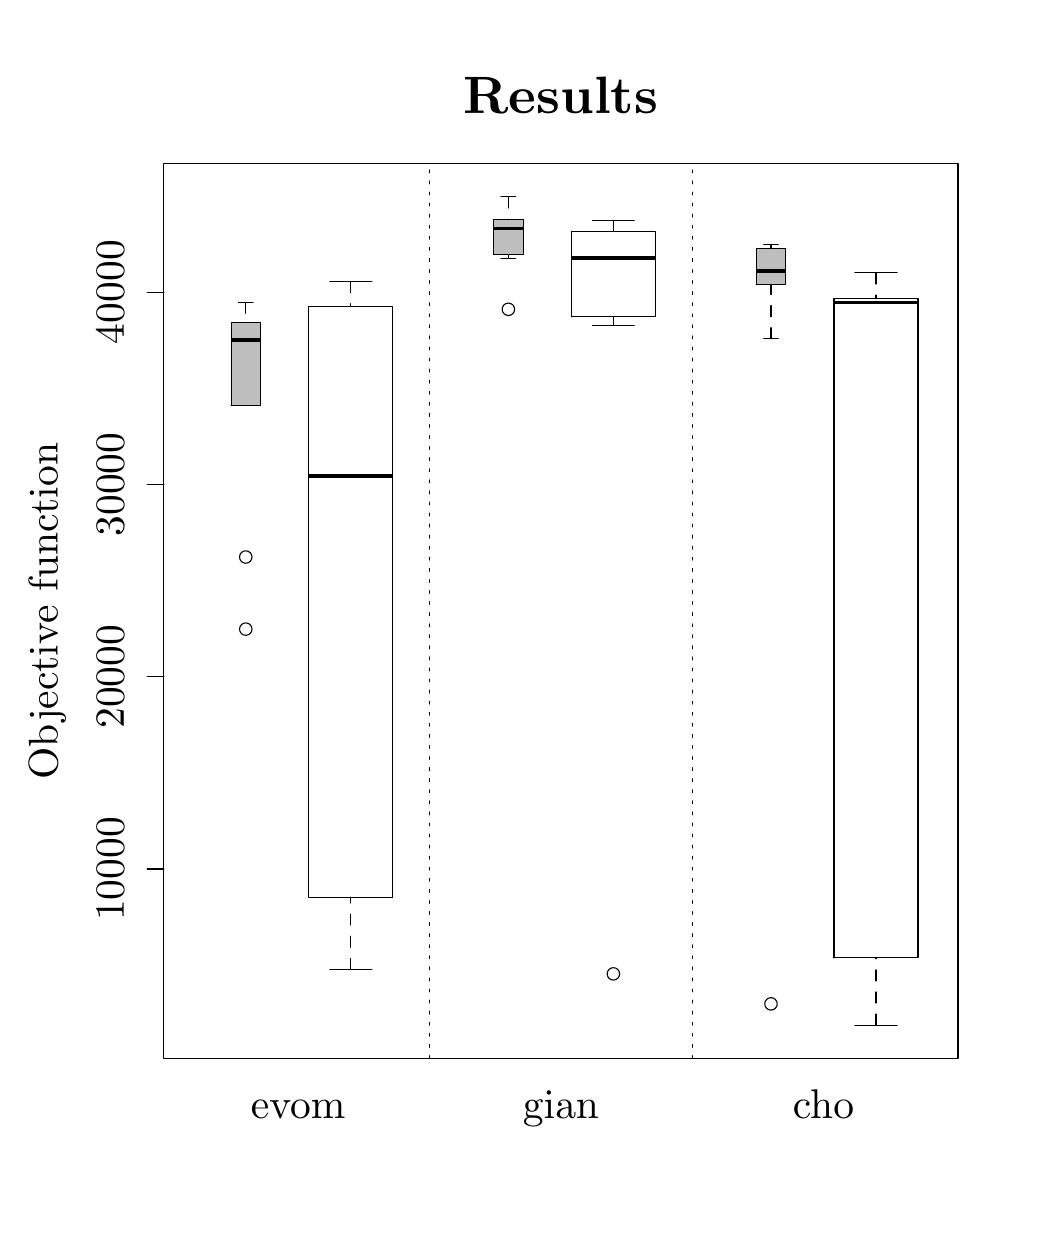
\begin{tikzpicture}[x=1pt,y=1pt]
\definecolor{fillColor}{RGB}{255,255,255}
\path[use as bounding box,fill=fillColor,fill opacity=0.00] (0,0) rectangle (361.35,433.62);
\begin{scope}
\path[clip] ( 49.20, 61.20) rectangle (336.15,384.42);
\definecolor{fillColor}{RGB}{190,190,190}

\path[fill=fillColor] ( 73.49,297.05) --
	( 84.12,297.05) --
	( 84.12,327.09) --
	( 73.49,327.09) --
	cycle;
\definecolor{drawColor}{RGB}{0,0,0}

\path[draw=drawColor,line width= 1.2pt,line join=round] ( 73.49,320.70) -- ( 84.12,320.70);

\path[draw=drawColor,line width= 0.4pt,dash pattern=on 4pt off 4pt ,line join=round,line cap=round] ( 78.81,297.05) -- ( 78.81,297.05);

\path[draw=drawColor,line width= 0.4pt,dash pattern=on 4pt off 4pt ,line join=round,line cap=round] ( 78.81,334.37) -- ( 78.81,327.09);

\path[draw=drawColor,line width= 0.4pt,line join=round,line cap=round] ( 76.15,297.05) -- ( 81.46,297.05);

\path[draw=drawColor,line width= 0.4pt,line join=round,line cap=round] ( 76.15,334.37) -- ( 81.46,334.37);

\path[draw=drawColor,line width= 0.4pt,line join=round,line cap=round] ( 73.49,297.05) --
	( 84.12,297.05) --
	( 84.12,327.09) --
	( 73.49,327.09) --
	( 73.49,297.05);

\path[draw=drawColor,line width= 0.4pt,line join=round,line cap=round] ( 78.81,242.33) circle (  2.25);

\path[draw=drawColor,line width= 0.4pt,line join=round,line cap=round] ( 78.81,216.29) circle (  2.25);
\definecolor{fillColor}{RGB}{255,255,255}

\path[fill=fillColor] (101.58,119.42) --
	(131.94,119.42) --
	(131.94,332.86) --
	(101.58,332.86) --
	cycle;

\path[draw=drawColor,line width= 1.2pt,line join=round] (101.58,271.60) -- (131.94,271.60);

\path[draw=drawColor,line width= 0.4pt,dash pattern=on 4pt off 4pt ,line join=round,line cap=round] (116.76, 93.32) -- (116.76,119.42);

\path[draw=drawColor,line width= 0.4pt,dash pattern=on 4pt off 4pt ,line join=round,line cap=round] (116.76,341.86) -- (116.76,332.86);

\path[draw=drawColor,line width= 0.4pt,line join=round,line cap=round] (109.17, 93.32) -- (124.35, 93.32);

\path[draw=drawColor,line width= 0.4pt,line join=round,line cap=round] (109.17,341.86) -- (124.35,341.86);

\path[draw=drawColor,line width= 0.4pt,line join=round,line cap=round] (101.58,119.42) --
	(131.94,119.42) --
	(131.94,332.86) --
	(101.58,332.86) --
	(101.58,119.42);
\definecolor{fillColor}{RGB}{190,190,190}

\path[fill=fillColor] (168.38,351.63) --
	(179.01,351.63) --
	(179.01,364.37) --
	(168.38,364.37) --
	cycle;

\path[draw=drawColor,line width= 1.2pt,line join=round] (168.38,361.13) -- (179.01,361.13);

\path[draw=drawColor,line width= 0.4pt,dash pattern=on 4pt off 4pt ,line join=round,line cap=round] (173.70,350.16) -- (173.70,351.63);

\path[draw=drawColor,line width= 0.4pt,dash pattern=on 4pt off 4pt ,line join=round,line cap=round] (173.70,372.45) -- (173.70,364.37);

\path[draw=drawColor,line width= 0.4pt,line join=round,line cap=round] (171.04,350.16) -- (176.35,350.16);

\path[draw=drawColor,line width= 0.4pt,line join=round,line cap=round] (171.04,372.45) -- (176.35,372.45);

\path[draw=drawColor,line width= 0.4pt,line join=round,line cap=round] (168.38,351.63) --
	(179.01,351.63) --
	(179.01,364.37) --
	(168.38,364.37) --
	(168.38,351.63);

\path[draw=drawColor,line width= 0.4pt,line join=round,line cap=round] (173.70,331.85) circle (  2.25);
\definecolor{fillColor}{RGB}{255,255,255}

\path[fill=fillColor] (196.47,329.15) --
	(226.84,329.15) --
	(226.84,359.82) --
	(196.47,359.82) --
	cycle;

\path[draw=drawColor,line width= 1.2pt,line join=round] (196.47,350.33) -- (226.84,350.33);

\path[draw=drawColor,line width= 0.4pt,dash pattern=on 4pt off 4pt ,line join=round,line cap=round] (211.65,326.04) -- (211.65,329.15);

\path[draw=drawColor,line width= 0.4pt,dash pattern=on 4pt off 4pt ,line join=round,line cap=round] (211.65,363.98) -- (211.65,359.82);

\path[draw=drawColor,line width= 0.4pt,line join=round,line cap=round] (204.06,326.04) -- (219.24,326.04);

\path[draw=drawColor,line width= 0.4pt,line join=round,line cap=round] (204.06,363.98) -- (219.24,363.98);

\path[draw=drawColor,line width= 0.4pt,line join=round,line cap=round] (196.47,329.15) --
	(226.84,329.15) --
	(226.84,359.82) --
	(196.47,359.82) --
	(196.47,329.15);

\path[draw=drawColor,line width= 0.4pt,line join=round,line cap=round] (211.65, 91.71) circle (  2.25);
\definecolor{fillColor}{RGB}{190,190,190}

\path[fill=fillColor] (263.27,340.73) --
	(273.90,340.73) --
	(273.90,353.79) --
	(263.27,353.79) --
	cycle;

\path[draw=drawColor,line width= 1.2pt,line join=round] (263.27,345.66) -- (273.90,345.66);

\path[draw=drawColor,line width= 0.4pt,dash pattern=on 4pt off 4pt ,line join=round,line cap=round] (268.59,321.20) -- (268.59,340.73);

\path[draw=drawColor,line width= 0.4pt,dash pattern=on 4pt off 4pt ,line join=round,line cap=round] (268.59,355.32) -- (268.59,353.79);

\path[draw=drawColor,line width= 0.4pt,line join=round,line cap=round] (265.93,321.20) -- (271.24,321.20);

\path[draw=drawColor,line width= 0.4pt,line join=round,line cap=round] (265.93,355.32) -- (271.24,355.32);

\path[draw=drawColor,line width= 0.4pt,line join=round,line cap=round] (263.27,340.73) --
	(273.90,340.73) --
	(273.90,353.79) --
	(263.27,353.79) --
	(263.27,340.73);

\path[draw=drawColor,line width= 0.4pt,line join=round,line cap=round] (268.59, 80.87) circle (  2.25);
\definecolor{fillColor}{RGB}{255,255,255}

\path[fill=fillColor] (291.36, 97.47) --
	(321.73, 97.47) --
	(321.73,335.67) --
	(291.36,335.67) --
	cycle;

\path[draw=drawColor,line width= 1.2pt,line join=round] (291.36,334.31) -- (321.73,334.31);

\path[draw=drawColor,line width= 0.4pt,dash pattern=on 4pt off 4pt ,line join=round,line cap=round] (306.54, 73.17) -- (306.54, 97.47);

\path[draw=drawColor,line width= 0.4pt,dash pattern=on 4pt off 4pt ,line join=round,line cap=round] (306.54,344.99) -- (306.54,335.67);

\path[draw=drawColor,line width= 0.4pt,line join=round,line cap=round] (298.95, 73.17) -- (314.14, 73.17);

\path[draw=drawColor,line width= 0.4pt,line join=round,line cap=round] (298.95,344.99) -- (314.14,344.99);

\path[draw=drawColor,line width= 0.4pt,line join=round,line cap=round] (291.36, 97.47) --
	(321.73, 97.47) --
	(321.73,335.67) --
	(291.36,335.67) --
	(291.36, 97.47);
\end{scope}
\begin{scope}
\path[clip] (  0.00,  0.00) rectangle (361.35,433.62);
\definecolor{drawColor}{RGB}{0,0,0}

\node[text=drawColor,rotate= 90.00,anchor=base,inner sep=0pt, outer sep=0pt, scale=  1.50] at ( 10.80,222.81) {Objective function};
\end{scope}
\begin{scope}
\path[clip] ( 49.20, 61.20) rectangle (336.15,384.42);
\definecolor{drawColor}{RGB}{0,0,0}

\path[draw=drawColor,line width= 0.4pt,dash pattern=on 1pt off 3pt ,line join=round,line cap=round] (145.23, 61.20) -- (145.23,384.42);

\path[draw=drawColor,line width= 0.4pt,dash pattern=on 1pt off 3pt ,line join=round,line cap=round] (240.12, 61.20) -- (240.12,384.42);
\end{scope}
\begin{scope}
\path[clip] (  0.00,  0.00) rectangle (361.35,433.62);
\definecolor{drawColor}{RGB}{0,0,0}

\node[text=drawColor,anchor=base,inner sep=0pt, outer sep=0pt, scale=  1.50] at ( 97.78, 39.60) {evom};

\node[text=drawColor,anchor=base,inner sep=0pt, outer sep=0pt, scale=  1.50] at (192.67, 39.60) {gian};

\node[text=drawColor,anchor=base,inner sep=0pt, outer sep=0pt, scale=  1.50] at (287.57, 39.60) {cho};
\end{scope}
\begin{scope}
\path[clip] (  0.00,  0.00) rectangle (361.35,433.62);
\definecolor{drawColor}{RGB}{0,0,0}

\node[text=drawColor,anchor=base,inner sep=0pt, outer sep=0pt, scale=  1.90] at (192.68,402.46) {\bfseries Results};
\end{scope}
\begin{scope}
\path[clip] (  0.00,  0.00) rectangle (361.35,433.62);
\definecolor{drawColor}{RGB}{0,0,0}

\path[draw=drawColor,line width= 0.4pt,line join=round,line cap=round] ( 49.20,129.62) -- ( 49.20,338.06);

\path[draw=drawColor,line width= 0.4pt,line join=round,line cap=round] ( 49.20,129.62) -- ( 43.20,129.62);

\path[draw=drawColor,line width= 0.4pt,line join=round,line cap=round] ( 49.20,199.10) -- ( 43.20,199.10);

\path[draw=drawColor,line width= 0.4pt,line join=round,line cap=round] ( 49.20,268.58) -- ( 43.20,268.58);

\path[draw=drawColor,line width= 0.4pt,line join=round,line cap=round] ( 49.20,338.06) -- ( 43.20,338.06);

\node[text=drawColor,rotate= 90.00,anchor=base,inner sep=0pt, outer sep=0pt, scale=  1.50] at ( 34.80,129.62) {10000};

\node[text=drawColor,rotate= 90.00,anchor=base,inner sep=0pt, outer sep=0pt, scale=  1.50] at ( 34.80,199.10) {20000};

\node[text=drawColor,rotate= 90.00,anchor=base,inner sep=0pt, outer sep=0pt, scale=  1.50] at ( 34.80,268.58) {30000};

\node[text=drawColor,rotate= 90.00,anchor=base,inner sep=0pt, outer sep=0pt, scale=  1.50] at ( 34.80,338.06) {40000};

\path[draw=drawColor,line width= 0.4pt,line join=round,line cap=round] ( 49.20, 61.20) --
	(336.15, 61.20) --
	(336.15,384.42) --
	( 49.20,384.42) --
	( 49.20, 61.20);
\end{scope}
\end{tikzpicture}

\hfill
% Created by tikzDevice version 0.11 on 2018-04-09 15:27:54
% !TEX encoding = UTF-8 Unicode
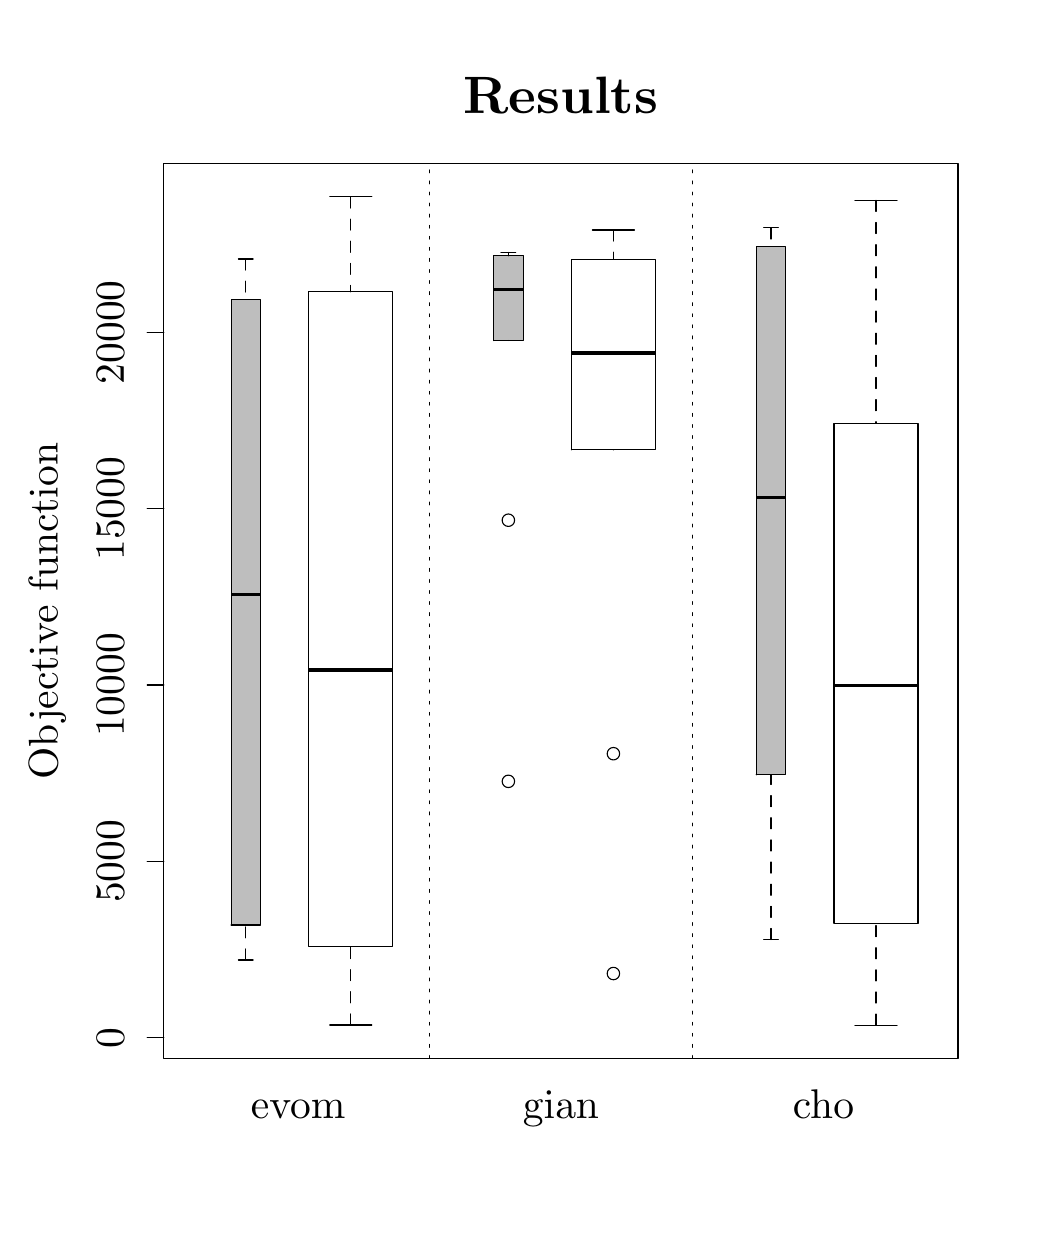
\begin{tikzpicture}[x=1pt,y=1pt]
\definecolor{fillColor}{RGB}{255,255,255}
\path[use as bounding box,fill=fillColor,fill opacity=0.00] (0,0) rectangle (361.35,433.62);
\begin{scope}
\path[clip] ( 49.20, 61.20) rectangle (336.15,384.42);
\definecolor{fillColor}{RGB}{190,190,190}

\path[fill=fillColor] ( 73.49,109.38) --
	( 84.12,109.38) --
	( 84.12,335.40) --
	( 73.49,335.40) --
	cycle;
\definecolor{drawColor}{RGB}{0,0,0}

\path[draw=drawColor,line width= 1.2pt,line join=round] ( 73.49,228.83) -- ( 84.12,228.83);

\path[draw=drawColor,line width= 0.4pt,dash pattern=on 4pt off 4pt ,line join=round,line cap=round] ( 78.81, 96.71) -- ( 78.81,109.38);

\path[draw=drawColor,line width= 0.4pt,dash pattern=on 4pt off 4pt ,line join=round,line cap=round] ( 78.81,350.04) -- ( 78.81,335.40);

\path[draw=drawColor,line width= 0.4pt,line join=round,line cap=round] ( 76.15, 96.71) -- ( 81.46, 96.71);

\path[draw=drawColor,line width= 0.4pt,line join=round,line cap=round] ( 76.15,350.04) -- ( 81.46,350.04);

\path[draw=drawColor,line width= 0.4pt,line join=round,line cap=round] ( 73.49,109.38) --
	( 84.12,109.38) --
	( 84.12,335.40) --
	( 73.49,335.40) --
	( 73.49,109.38);
\definecolor{fillColor}{RGB}{255,255,255}

\path[fill=fillColor] (101.58,101.70) --
	(131.94,101.70) --
	(131.94,338.19) --
	(101.58,338.19) --
	cycle;

\path[draw=drawColor,line width= 1.2pt,line join=round] (101.58,201.56) -- (131.94,201.56);

\path[draw=drawColor,line width= 0.4pt,dash pattern=on 4pt off 4pt ,line join=round,line cap=round] (116.76, 73.25) -- (116.76,101.70);

\path[draw=drawColor,line width= 0.4pt,dash pattern=on 4pt off 4pt ,line join=round,line cap=round] (116.76,372.45) -- (116.76,338.19);

\path[draw=drawColor,line width= 0.4pt,line join=round,line cap=round] (109.17, 73.25) -- (124.35, 73.25);

\path[draw=drawColor,line width= 0.4pt,line join=round,line cap=round] (109.17,372.45) -- (124.35,372.45);

\path[draw=drawColor,line width= 0.4pt,line join=round,line cap=round] (101.58,101.70) --
	(131.94,101.70) --
	(131.94,338.19) --
	(101.58,338.19) --
	(101.58,101.70);
\definecolor{fillColor}{RGB}{190,190,190}

\path[fill=fillColor] (168.38,320.56) --
	(179.01,320.56) --
	(179.01,351.13) --
	(168.38,351.13) --
	cycle;

\path[draw=drawColor,line width= 1.2pt,line join=round] (168.38,338.97) -- (179.01,338.97);

\path[draw=drawColor,line width= 0.4pt,dash pattern=on 4pt off 4pt ,line join=round,line cap=round] (173.70,320.56) -- (173.70,320.56);

\path[draw=drawColor,line width= 0.4pt,dash pattern=on 4pt off 4pt ,line join=round,line cap=round] (173.70,352.37) -- (173.70,351.13);

\path[draw=drawColor,line width= 0.4pt,line join=round,line cap=round] (171.04,320.56) -- (176.35,320.56);

\path[draw=drawColor,line width= 0.4pt,line join=round,line cap=round] (171.04,352.37) -- (176.35,352.37);

\path[draw=drawColor,line width= 0.4pt,line join=round,line cap=round] (168.38,320.56) --
	(179.01,320.56) --
	(179.01,351.13) --
	(168.38,351.13) --
	(168.38,320.56);

\path[draw=drawColor,line width= 0.4pt,line join=round,line cap=round] (173.70,255.64) circle (  2.25);

\path[draw=drawColor,line width= 0.4pt,line join=round,line cap=round] (173.70,161.28) circle (  2.25);
\definecolor{fillColor}{RGB}{255,255,255}

\path[fill=fillColor] (196.47,281.03) --
	(226.84,281.03) --
	(226.84,349.91) --
	(196.47,349.91) --
	cycle;

\path[draw=drawColor,line width= 1.2pt,line join=round] (196.47,316.10) -- (226.84,316.10);

\path[draw=drawColor,line width= 0.4pt,dash pattern=on 4pt off 4pt ,line join=round,line cap=round] (211.65,281.03) -- (211.65,281.03);

\path[draw=drawColor,line width= 0.4pt,dash pattern=on 4pt off 4pt ,line join=round,line cap=round] (211.65,360.49) -- (211.65,349.91);

\path[draw=drawColor,line width= 0.4pt,line join=round,line cap=round] (204.06,281.03) -- (219.24,281.03);

\path[draw=drawColor,line width= 0.4pt,line join=round,line cap=round] (204.06,360.49) -- (219.24,360.49);

\path[draw=drawColor,line width= 0.4pt,line join=round,line cap=round] (196.47,281.03) --
	(226.84,281.03) --
	(226.84,349.91) --
	(196.47,349.91) --
	(196.47,281.03);

\path[draw=drawColor,line width= 0.4pt,line join=round,line cap=round] (211.65, 91.83) circle (  2.25);

\path[draw=drawColor,line width= 0.4pt,line join=round,line cap=round] (211.65,171.27) circle (  2.25);
\definecolor{fillColor}{RGB}{190,190,190}

\path[fill=fillColor] (263.27,163.60) --
	(273.90,163.60) --
	(273.90,354.52) --
	(263.27,354.52) --
	cycle;

\path[draw=drawColor,line width= 1.2pt,line join=round] (263.27,263.84) -- (273.90,263.84);

\path[draw=drawColor,line width= 0.4pt,dash pattern=on 4pt off 4pt ,line join=round,line cap=round] (268.59,104.12) -- (268.59,163.60);

\path[draw=drawColor,line width= 0.4pt,dash pattern=on 4pt off 4pt ,line join=round,line cap=round] (268.59,361.25) -- (268.59,354.52);

\path[draw=drawColor,line width= 0.4pt,line join=round,line cap=round] (265.93,104.12) -- (271.24,104.12);

\path[draw=drawColor,line width= 0.4pt,line join=round,line cap=round] (265.93,361.25) -- (271.24,361.25);

\path[draw=drawColor,line width= 0.4pt,line join=round,line cap=round] (263.27,163.60) --
	(273.90,163.60) --
	(273.90,354.52) --
	(263.27,354.52) --
	(263.27,163.60);
\definecolor{fillColor}{RGB}{255,255,255}

\path[fill=fillColor] (291.36,110.06) --
	(321.73,110.06) --
	(321.73,290.69) --
	(291.36,290.69) --
	cycle;

\path[draw=drawColor,line width= 1.2pt,line join=round] (291.36,196.02) -- (321.73,196.02);

\path[draw=drawColor,line width= 0.4pt,dash pattern=on 4pt off 4pt ,line join=round,line cap=round] (306.54, 73.17) -- (306.54,110.06);

\path[draw=drawColor,line width= 0.4pt,dash pattern=on 4pt off 4pt ,line join=round,line cap=round] (306.54,371.21) -- (306.54,290.69);

\path[draw=drawColor,line width= 0.4pt,line join=round,line cap=round] (298.95, 73.17) -- (314.14, 73.17);

\path[draw=drawColor,line width= 0.4pt,line join=round,line cap=round] (298.95,371.21) -- (314.14,371.21);

\path[draw=drawColor,line width= 0.4pt,line join=round,line cap=round] (291.36,110.06) --
	(321.73,110.06) --
	(321.73,290.69) --
	(291.36,290.69) --
	(291.36,110.06);
\end{scope}
\begin{scope}
\path[clip] (  0.00,  0.00) rectangle (361.35,433.62);
\definecolor{drawColor}{RGB}{0,0,0}

\node[text=drawColor,rotate= 90.00,anchor=base,inner sep=0pt, outer sep=0pt, scale=  1.50] at ( 10.80,222.81) {Objective function};
\end{scope}
\begin{scope}
\path[clip] ( 49.20, 61.20) rectangle (336.15,384.42);
\definecolor{drawColor}{RGB}{0,0,0}

\path[draw=drawColor,line width= 0.4pt,dash pattern=on 1pt off 3pt ,line join=round,line cap=round] (145.23, 61.20) -- (145.23,384.42);

\path[draw=drawColor,line width= 0.4pt,dash pattern=on 1pt off 3pt ,line join=round,line cap=round] (240.12, 61.20) -- (240.12,384.42);
\end{scope}
\begin{scope}
\path[clip] (  0.00,  0.00) rectangle (361.35,433.62);
\definecolor{drawColor}{RGB}{0,0,0}

\node[text=drawColor,anchor=base,inner sep=0pt, outer sep=0pt, scale=  1.50] at ( 97.78, 39.60) {evom};

\node[text=drawColor,anchor=base,inner sep=0pt, outer sep=0pt, scale=  1.50] at (192.67, 39.60) {gian};

\node[text=drawColor,anchor=base,inner sep=0pt, outer sep=0pt, scale=  1.50] at (287.57, 39.60) {cho};
\end{scope}
\begin{scope}
\path[clip] (  0.00,  0.00) rectangle (361.35,433.62);
\definecolor{drawColor}{RGB}{0,0,0}

\node[text=drawColor,anchor=base,inner sep=0pt, outer sep=0pt, scale=  1.90] at (192.68,402.46) {\bfseries Results};
\end{scope}
\begin{scope}
\path[clip] (  0.00,  0.00) rectangle (361.35,433.62);
\definecolor{drawColor}{RGB}{0,0,0}

\path[draw=drawColor,line width= 0.4pt,line join=round,line cap=round] ( 49.20, 68.62) -- ( 49.20,323.53);

\path[draw=drawColor,line width= 0.4pt,line join=round,line cap=round] ( 49.20, 68.62) -- ( 43.20, 68.62);

\path[draw=drawColor,line width= 0.4pt,line join=round,line cap=round] ( 49.20,132.35) -- ( 43.20,132.35);

\path[draw=drawColor,line width= 0.4pt,line join=round,line cap=round] ( 49.20,196.08) -- ( 43.20,196.08);

\path[draw=drawColor,line width= 0.4pt,line join=round,line cap=round] ( 49.20,259.80) -- ( 43.20,259.80);

\path[draw=drawColor,line width= 0.4pt,line join=round,line cap=round] ( 49.20,323.53) -- ( 43.20,323.53);

\node[text=drawColor,rotate= 90.00,anchor=base,inner sep=0pt, outer sep=0pt, scale=  1.50] at ( 34.80, 68.62) {0};

\node[text=drawColor,rotate= 90.00,anchor=base,inner sep=0pt, outer sep=0pt, scale=  1.50] at ( 34.80,132.35) {5000};

\node[text=drawColor,rotate= 90.00,anchor=base,inner sep=0pt, outer sep=0pt, scale=  1.50] at ( 34.80,196.08) {10000};

\node[text=drawColor,rotate= 90.00,anchor=base,inner sep=0pt, outer sep=0pt, scale=  1.50] at ( 34.80,259.80) {15000};

\node[text=drawColor,rotate= 90.00,anchor=base,inner sep=0pt, outer sep=0pt, scale=  1.50] at ( 34.80,323.53) {20000};

\path[draw=drawColor,line width= 0.4pt,line join=round,line cap=round] ( 49.20, 61.20) --
	(336.15, 61.20) --
	(336.15,384.42) --
	( 49.20,384.42) --
	( 49.20, 61.20);
\end{scope}
\end{tikzpicture}

\caption{
Thick gray boxes represent the results of robot experiments;
Thick white boxes those of pseudo-reality; thin gray ones,
those of simulations.}
\label{fig:task1res}
\end{figure}

\begin{figure}[t]
\centering
% Created by tikzDevice version 0.12 on 2019-02-08 11:09:25
% !TEX encoding = UTF-8 Unicode
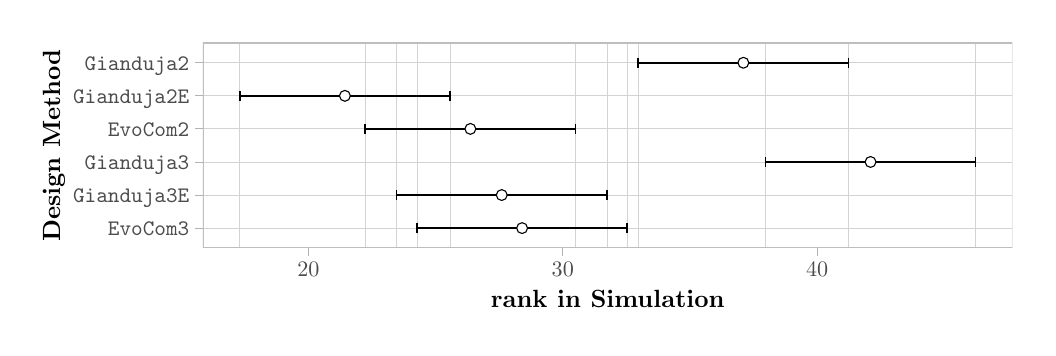
\begin{tikzpicture}[x=1pt,y=1pt]
\definecolor{fillColor}{RGB}{255,255,255}
\path[use as bounding box,fill=fillColor,fill opacity=0.00] (0,0) rectangle (361.35,108.41);
\begin{scope}
\path[clip] (  0.00,  0.00) rectangle (361.35,108.40);
\definecolor{drawColor}{RGB}{255,255,255}
\definecolor{fillColor}{RGB}{255,255,255}

\path[draw=drawColor,line width= 0.6pt,line join=round,line cap=round,fill=fillColor] (  0.00,  0.00) rectangle (361.35,108.40);
\end{scope}
\begin{scope}
\path[clip] ( 63.34, 28.81) rectangle (355.85,102.90);
\definecolor{fillColor}{RGB}{255,255,255}

\path[fill=fillColor] ( 63.34, 28.81) rectangle (355.85,102.90);
\definecolor{drawColor}{RGB}{211,211,211}

\path[draw=drawColor,line width= 0.3pt,line join=round] ( 63.34, 71.83) --
	(355.85, 71.83);

\path[draw=drawColor,line width= 0.3pt,line join=round] ( 63.34, 35.98) --
	(355.85, 35.98);

\path[draw=drawColor,line width= 0.3pt,line join=round] ( 63.34, 95.73) --
	(355.85, 95.73);

\path[draw=drawColor,line width= 0.3pt,line join=round] ( 63.34, 83.78) --
	(355.85, 83.78);

\path[draw=drawColor,line width= 0.3pt,line join=round] ( 63.34, 59.88) --
	(355.85, 59.88);

\path[draw=drawColor,line width= 0.3pt,line join=round] ( 63.34, 47.93) --
	(355.85, 47.93);

\path[draw=drawColor,line width= 0.2pt,line join=round] (197.95, 28.81) -- (197.95,102.90);

\path[draw=drawColor,line width= 0.2pt,line join=round] (296.60, 28.81) -- (296.60,102.90);

\path[draw=drawColor,line width= 0.2pt,line join=round] (152.61, 28.81) -- (152.61,102.90);

\path[draw=drawColor,line width= 0.2pt,line join=round] (216.64, 28.81) -- (216.64,102.90);

\path[draw=drawColor,line width= 0.2pt,line join=round] (342.55, 28.81) -- (342.55,102.90);

\path[draw=drawColor,line width= 0.2pt,line join=round] (209.29, 28.81) -- (209.29,102.90);

\path[draw=drawColor,line width= 0.2pt,line join=round] (121.98, 28.81) -- (121.98,102.90);

\path[draw=drawColor,line width= 0.2pt,line join=round] (220.63, 28.81) -- (220.63,102.90);

\path[draw=drawColor,line width= 0.2pt,line join=round] ( 76.64, 28.81) -- ( 76.64,102.90);

\path[draw=drawColor,line width= 0.2pt,line join=round] (140.67, 28.81) -- (140.67,102.90);

\path[draw=drawColor,line width= 0.2pt,line join=round] (266.58, 28.81) -- (266.58,102.90);

\path[draw=drawColor,line width= 0.2pt,line join=round] (133.32, 28.81) -- (133.32,102.90);
\definecolor{drawColor}{RGB}{0,0,0}

\path[draw=drawColor,line width= 0.6pt,line join=round] (197.95, 70.04) --
	(197.95, 73.62);

\path[draw=drawColor,line width= 0.6pt,line join=round] (197.95, 71.83) --
	(121.98, 71.83);

\path[draw=drawColor,line width= 0.6pt,line join=round] (121.98, 70.04) --
	(121.98, 73.62);

\path[draw=drawColor,line width= 0.6pt,line join=round] (296.60, 93.94) --
	(296.60, 97.53);

\path[draw=drawColor,line width= 0.6pt,line join=round] (296.60, 95.73) --
	(220.63, 95.73);

\path[draw=drawColor,line width= 0.6pt,line join=round] (220.63, 93.94) --
	(220.63, 97.53);

\path[draw=drawColor,line width= 0.6pt,line join=round] (152.61, 81.99) --
	(152.61, 85.58);

\path[draw=drawColor,line width= 0.6pt,line join=round] (152.61, 83.78) --
	( 76.64, 83.78);

\path[draw=drawColor,line width= 0.6pt,line join=round] ( 76.64, 81.99) --
	( 76.64, 85.58);

\path[draw=drawColor,line width= 0.6pt,line join=round] (216.64, 34.19) --
	(216.64, 37.77);

\path[draw=drawColor,line width= 0.6pt,line join=round] (216.64, 35.98) --
	(140.67, 35.98);

\path[draw=drawColor,line width= 0.6pt,line join=round] (140.67, 34.19) --
	(140.67, 37.77);

\path[draw=drawColor,line width= 0.6pt,line join=round] (342.55, 58.09) --
	(342.55, 61.67);

\path[draw=drawColor,line width= 0.6pt,line join=round] (342.55, 59.88) --
	(266.58, 59.88);

\path[draw=drawColor,line width= 0.6pt,line join=round] (266.58, 58.09) --
	(266.58, 61.67);

\path[draw=drawColor,line width= 0.6pt,line join=round] (209.29, 46.14) --
	(209.29, 49.72);

\path[draw=drawColor,line width= 0.6pt,line join=round] (209.29, 47.93) --
	(133.32, 47.93);

\path[draw=drawColor,line width= 0.6pt,line join=round] (133.32, 46.14) --
	(133.32, 49.72);

\path[draw=drawColor,line width= 0.4pt,line join=round,line cap=round,fill=fillColor] (159.97, 71.83) circle (  1.96);

\path[draw=drawColor,line width= 0.4pt,line join=round,line cap=round,fill=fillColor] (258.62, 95.73) circle (  1.96);

\path[draw=drawColor,line width= 0.4pt,line join=round,line cap=round,fill=fillColor] (114.63, 83.78) circle (  1.96);

\path[draw=drawColor,line width= 0.4pt,line join=round,line cap=round,fill=fillColor] (178.66, 35.98) circle (  1.96);

\path[draw=drawColor,line width= 0.4pt,line join=round,line cap=round,fill=fillColor] (304.57, 59.88) circle (  1.96);

\path[draw=drawColor,line width= 0.4pt,line join=round,line cap=round,fill=fillColor] (171.30, 47.93) circle (  1.96);
\definecolor{drawColor}{RGB}{190,190,190}

\path[draw=drawColor,line width= 0.6pt,line join=round,line cap=round] ( 63.34, 28.81) rectangle (355.85,102.90);
\end{scope}
\begin{scope}
\path[clip] (  0.00,  0.00) rectangle (361.35,108.41);
\definecolor{drawColor}{gray}{0.30}

\node[text=drawColor,anchor=base east,inner sep=0pt, outer sep=0pt, scale=  0.80] at ( 58.39, 69.08) {\texttt{EvoCom2}};

\node[text=drawColor,anchor=base east,inner sep=0pt, outer sep=0pt, scale=  0.80] at ( 58.39, 33.22) {\texttt{EvoCom3}};

\node[text=drawColor,anchor=base east,inner sep=0pt, outer sep=0pt, scale=  0.80] at ( 58.39, 92.98) {\texttt{Gianduja2}};

\node[text=drawColor,anchor=base east,inner sep=0pt, outer sep=0pt, scale=  0.80] at ( 58.39, 81.03) {\texttt{Gianduja2E}};

\node[text=drawColor,anchor=base east,inner sep=0pt, outer sep=0pt, scale=  0.80] at ( 58.39, 57.13) {\texttt{Gianduja3}};

\node[text=drawColor,anchor=base east,inner sep=0pt, outer sep=0pt, scale=  0.80] at ( 58.39, 45.18) {\texttt{Gianduja3E}};
\end{scope}
\begin{scope}
\path[clip] (  0.00,  0.00) rectangle (361.35,108.41);
\definecolor{drawColor}{gray}{0.70}

\path[draw=drawColor,line width= 0.3pt,line join=round] ( 60.59, 71.83) --
	( 63.34, 71.83);

\path[draw=drawColor,line width= 0.3pt,line join=round] ( 60.59, 35.98) --
	( 63.34, 35.98);

\path[draw=drawColor,line width= 0.3pt,line join=round] ( 60.59, 95.73) --
	( 63.34, 95.73);

\path[draw=drawColor,line width= 0.3pt,line join=round] ( 60.59, 83.78) --
	( 63.34, 83.78);

\path[draw=drawColor,line width= 0.3pt,line join=round] ( 60.59, 59.88) --
	( 63.34, 59.88);

\path[draw=drawColor,line width= 0.3pt,line join=round] ( 60.59, 47.93) --
	( 63.34, 47.93);
\end{scope}
\begin{scope}
\path[clip] (  0.00,  0.00) rectangle (361.35,108.41);
\definecolor{drawColor}{gray}{0.70}

\path[draw=drawColor,line width= 0.3pt,line join=round] (101.45, 26.06) --
	(101.45, 28.81);

\path[draw=drawColor,line width= 0.3pt,line join=round] (193.36, 26.06) --
	(193.36, 28.81);

\path[draw=drawColor,line width= 0.3pt,line join=round] (285.27, 26.06) --
	(285.27, 28.81);
\end{scope}
\begin{scope}
\path[clip] (  0.00,  0.00) rectangle (361.35,108.41);
\definecolor{drawColor}{gray}{0.30}

\node[text=drawColor,anchor=base,inner sep=0pt, outer sep=0pt, scale=  0.80] at (101.45, 18.35) {20};

\node[text=drawColor,anchor=base,inner sep=0pt, outer sep=0pt, scale=  0.80] at (193.36, 18.35) {30};

\node[text=drawColor,anchor=base,inner sep=0pt, outer sep=0pt, scale=  0.80] at (285.27, 18.35) {40};
\end{scope}
\begin{scope}
\path[clip] (  0.00,  0.00) rectangle (361.35,108.41);
\definecolor{drawColor}{RGB}{0,0,0}

\node[text=drawColor,anchor=base,inner sep=0pt, outer sep=0pt, scale=  0.90] at (209.60,  7.44) {\bfseries rank in Simulation};
\end{scope}
\begin{scope}
\path[clip] (  0.00,  0.00) rectangle (361.35,108.41);
\definecolor{drawColor}{RGB}{0,0,0}

\node[text=drawColor,rotate= 90.00,anchor=base,inner sep=0pt, outer sep=0pt, scale=  0.90] at ( 11.71, 65.86) {\bfseries Design Method};
\end{scope}
\end{tikzpicture}

\caption{Friedman test on the aggregated results of the three missions. The
  plot represents the average rank of the seven methods and their
  95\% confidence interval. }
\label{fig:friedmanSIM}
\end{figure}

\begin{figure}[t]
\centering
% Created by tikzDevice version 0.12 on 2019-01-19 16:45:08
% !TEX encoding = UTF-8 Unicode
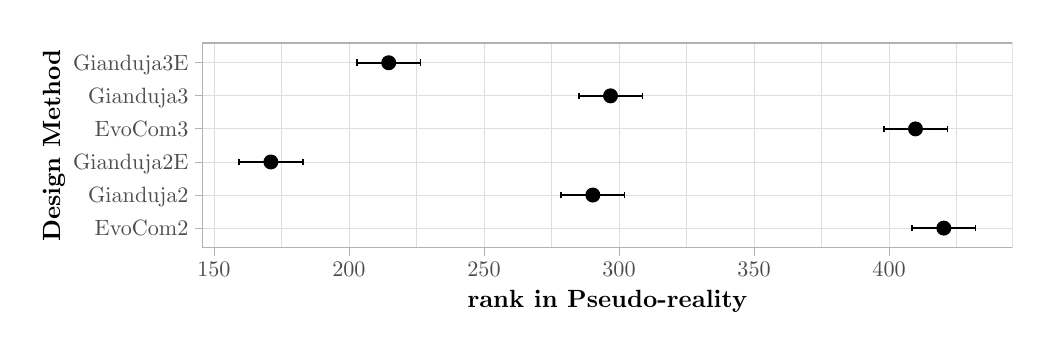
\begin{tikzpicture}[x=1pt,y=1pt]
\definecolor{fillColor}{RGB}{255,255,255}
\path[use as bounding box,fill=fillColor,fill opacity=0.00] (0,0) rectangle (361.35,108.41);
\begin{scope}
\path[clip] (  0.00,  0.00) rectangle (361.35,108.40);
\definecolor{drawColor}{RGB}{255,255,255}
\definecolor{fillColor}{RGB}{255,255,255}

\path[draw=drawColor,line width= 0.6pt,line join=round,line cap=round,fill=fillColor] (  0.00,  0.00) rectangle (361.35,108.40);
\end{scope}
\begin{scope}
\path[clip] ( 63.07, 28.81) rectangle (355.85,102.90);
\definecolor{fillColor}{RGB}{255,255,255}

\path[fill=fillColor] ( 63.07, 28.81) rectangle (355.85,102.90);
\definecolor{drawColor}{gray}{0.87}

\path[draw=drawColor,line width= 0.1pt,line join=round] ( 91.69, 28.81) --
	( 91.69,102.90);

\path[draw=drawColor,line width= 0.1pt,line join=round] (140.49, 28.81) --
	(140.49,102.90);

\path[draw=drawColor,line width= 0.1pt,line join=round] (189.28, 28.81) --
	(189.28,102.90);

\path[draw=drawColor,line width= 0.1pt,line join=round] (238.08, 28.81) --
	(238.08,102.90);

\path[draw=drawColor,line width= 0.1pt,line join=round] (286.87, 28.81) --
	(286.87,102.90);

\path[draw=drawColor,line width= 0.1pt,line join=round] (335.67, 28.81) --
	(335.67,102.90);

\path[draw=drawColor,line width= 0.3pt,line join=round] ( 63.07, 35.98) --
	(355.85, 35.98);

\path[draw=drawColor,line width= 0.3pt,line join=round] ( 63.07, 47.93) --
	(355.85, 47.93);

\path[draw=drawColor,line width= 0.3pt,line join=round] ( 63.07, 59.88) --
	(355.85, 59.88);

\path[draw=drawColor,line width= 0.3pt,line join=round] ( 63.07, 71.83) --
	(355.85, 71.83);

\path[draw=drawColor,line width= 0.3pt,line join=round] ( 63.07, 83.78) --
	(355.85, 83.78);

\path[draw=drawColor,line width= 0.3pt,line join=round] ( 63.07, 95.73) --
	(355.85, 95.73);

\path[draw=drawColor,line width= 0.3pt,line join=round] ( 67.30, 28.81) --
	( 67.30,102.90);

\path[draw=drawColor,line width= 0.3pt,line join=round] (116.09, 28.81) --
	(116.09,102.90);

\path[draw=drawColor,line width= 0.3pt,line join=round] (164.89, 28.81) --
	(164.89,102.90);

\path[draw=drawColor,line width= 0.3pt,line join=round] (213.68, 28.81) --
	(213.68,102.90);

\path[draw=drawColor,line width= 0.3pt,line join=round] (262.48, 28.81) --
	(262.48,102.90);

\path[draw=drawColor,line width= 0.3pt,line join=round] (311.27, 28.81) --
	(311.27,102.90);
\definecolor{drawColor}{RGB}{0,0,0}
\definecolor{fillColor}{RGB}{0,0,0}

\path[draw=drawColor,line width= 0.4pt,line join=round,line cap=round,fill=fillColor] (331.04, 35.98) circle (  2.50);

\path[draw=drawColor,line width= 0.4pt,line join=round,line cap=round,fill=fillColor] (204.22, 47.93) circle (  2.50);

\path[draw=drawColor,line width= 0.4pt,line join=round,line cap=round,fill=fillColor] ( 87.88, 59.88) circle (  2.50);

\path[draw=drawColor,line width= 0.4pt,line join=round,line cap=round,fill=fillColor] (320.81, 71.83) circle (  2.50);

\path[draw=drawColor,line width= 0.4pt,line join=round,line cap=round,fill=fillColor] (210.61, 83.78) circle (  2.50);

\path[draw=drawColor,line width= 0.4pt,line join=round,line cap=round,fill=fillColor] (130.45, 95.73) circle (  2.50);

\path[draw=drawColor,line width= 0.6pt,line join=round] (342.54, 34.78) --
	(342.54, 37.17);

\path[draw=drawColor,line width= 0.6pt,line join=round] (342.54, 35.98) --
	(319.54, 35.98);

\path[draw=drawColor,line width= 0.6pt,line join=round] (319.54, 34.78) --
	(319.54, 37.17);

\path[draw=drawColor,line width= 0.6pt,line join=round] (215.72, 46.74) --
	(215.72, 49.13);

\path[draw=drawColor,line width= 0.6pt,line join=round] (215.72, 47.93) --
	(192.72, 47.93);

\path[draw=drawColor,line width= 0.6pt,line join=round] (192.72, 46.74) --
	(192.72, 49.13);

\path[draw=drawColor,line width= 0.6pt,line join=round] ( 99.38, 58.69) --
	( 99.38, 61.08);

\path[draw=drawColor,line width= 0.6pt,line join=round] ( 99.38, 59.88) --
	( 76.38, 59.88);

\path[draw=drawColor,line width= 0.6pt,line join=round] ( 76.38, 58.69) --
	( 76.38, 61.08);

\path[draw=drawColor,line width= 0.6pt,line join=round] (332.32, 70.64) --
	(332.32, 73.03);

\path[draw=drawColor,line width= 0.6pt,line join=round] (332.32, 71.83) --
	(309.31, 71.83);

\path[draw=drawColor,line width= 0.6pt,line join=round] (309.31, 70.64) --
	(309.31, 73.03);

\path[draw=drawColor,line width= 0.6pt,line join=round] (222.11, 82.59) --
	(222.11, 84.98);

\path[draw=drawColor,line width= 0.6pt,line join=round] (222.11, 83.78) --
	(199.11, 83.78);

\path[draw=drawColor,line width= 0.6pt,line join=round] (199.11, 82.59) --
	(199.11, 84.98);

\path[draw=drawColor,line width= 0.6pt,line join=round] (141.95, 94.54) --
	(141.95, 96.93);

\path[draw=drawColor,line width= 0.6pt,line join=round] (141.95, 95.73) --
	(118.95, 95.73);

\path[draw=drawColor,line width= 0.6pt,line join=round] (118.95, 94.54) --
	(118.95, 96.93);
\definecolor{drawColor}{gray}{0.70}

\path[draw=drawColor,line width= 0.6pt,line join=round,line cap=round] ( 63.07, 28.81) rectangle (355.85,102.90);
\end{scope}
\begin{scope}
\path[clip] (  0.00,  0.00) rectangle (361.35,108.41);
\definecolor{drawColor}{gray}{0.30}

\node[text=drawColor,anchor=base east,inner sep=0pt, outer sep=0pt, scale=  0.80] at ( 58.12, 33.22) {EvoCom2};

\node[text=drawColor,anchor=base east,inner sep=0pt, outer sep=0pt, scale=  0.80] at ( 58.12, 45.18) {Gianduja2};

\node[text=drawColor,anchor=base east,inner sep=0pt, outer sep=0pt, scale=  0.80] at ( 58.12, 57.13) {Gianduja2E};

\node[text=drawColor,anchor=base east,inner sep=0pt, outer sep=0pt, scale=  0.80] at ( 58.12, 69.08) {EvoCom3};

\node[text=drawColor,anchor=base east,inner sep=0pt, outer sep=0pt, scale=  0.80] at ( 58.12, 81.03) {Gianduja3};

\node[text=drawColor,anchor=base east,inner sep=0pt, outer sep=0pt, scale=  0.80] at ( 58.12, 92.98) {Gianduja3E};
\end{scope}
\begin{scope}
\path[clip] (  0.00,  0.00) rectangle (361.35,108.41);
\definecolor{drawColor}{gray}{0.70}

\path[draw=drawColor,line width= 0.3pt,line join=round] ( 60.32, 35.98) --
	( 63.07, 35.98);

\path[draw=drawColor,line width= 0.3pt,line join=round] ( 60.32, 47.93) --
	( 63.07, 47.93);

\path[draw=drawColor,line width= 0.3pt,line join=round] ( 60.32, 59.88) --
	( 63.07, 59.88);

\path[draw=drawColor,line width= 0.3pt,line join=round] ( 60.32, 71.83) --
	( 63.07, 71.83);

\path[draw=drawColor,line width= 0.3pt,line join=round] ( 60.32, 83.78) --
	( 63.07, 83.78);

\path[draw=drawColor,line width= 0.3pt,line join=round] ( 60.32, 95.73) --
	( 63.07, 95.73);
\end{scope}
\begin{scope}
\path[clip] (  0.00,  0.00) rectangle (361.35,108.41);
\definecolor{drawColor}{gray}{0.70}

\path[draw=drawColor,line width= 0.3pt,line join=round] ( 67.30, 26.06) --
	( 67.30, 28.81);

\path[draw=drawColor,line width= 0.3pt,line join=round] (116.09, 26.06) --
	(116.09, 28.81);

\path[draw=drawColor,line width= 0.3pt,line join=round] (164.89, 26.06) --
	(164.89, 28.81);

\path[draw=drawColor,line width= 0.3pt,line join=round] (213.68, 26.06) --
	(213.68, 28.81);

\path[draw=drawColor,line width= 0.3pt,line join=round] (262.48, 26.06) --
	(262.48, 28.81);

\path[draw=drawColor,line width= 0.3pt,line join=round] (311.27, 26.06) --
	(311.27, 28.81);
\end{scope}
\begin{scope}
\path[clip] (  0.00,  0.00) rectangle (361.35,108.41);
\definecolor{drawColor}{gray}{0.30}

\node[text=drawColor,anchor=base,inner sep=0pt, outer sep=0pt, scale=  0.80] at ( 67.30, 18.35) {150};

\node[text=drawColor,anchor=base,inner sep=0pt, outer sep=0pt, scale=  0.80] at (116.09, 18.35) {200};

\node[text=drawColor,anchor=base,inner sep=0pt, outer sep=0pt, scale=  0.80] at (164.89, 18.35) {250};

\node[text=drawColor,anchor=base,inner sep=0pt, outer sep=0pt, scale=  0.80] at (213.68, 18.35) {300};

\node[text=drawColor,anchor=base,inner sep=0pt, outer sep=0pt, scale=  0.80] at (262.48, 18.35) {350};

\node[text=drawColor,anchor=base,inner sep=0pt, outer sep=0pt, scale=  0.80] at (311.27, 18.35) {400};
\end{scope}
\begin{scope}
\path[clip] (  0.00,  0.00) rectangle (361.35,108.41);
\definecolor{drawColor}{RGB}{0,0,0}

\node[text=drawColor,anchor=base,inner sep=0pt, outer sep=0pt, scale=  0.90] at (209.46,  7.44) {\bfseries rank in Pseudo-reality};
\end{scope}
\begin{scope}
\path[clip] (  0.00,  0.00) rectangle (361.35,108.41);
\definecolor{drawColor}{RGB}{0,0,0}

\node[text=drawColor,rotate= 90.00,anchor=base,inner sep=0pt, outer sep=0pt, scale=  0.90] at ( 11.71, 65.86) {\bfseries Design Method};
\end{scope}
\end{tikzpicture}

\caption{Friedman test on the aggregated results of the three missions. The
  plot represents the average rank of the seven methods and their
  95\% confidence interval. }
\label{fig:friedmanPR}
\end{figure}


\end{document}
